\documentclass[tikz, border=5pt]{standalone}

% Semantic GitHub colors for the light theme.
% The Poe task embeds the dark palette from theme-dark.css into each SVG.
\usepackage{tikz}
\usepackage{amsmath, amssymb}
\usetikzlibrary{arrows.meta, calc, positioning, decorations.pathreplacing}

% Text and surfaces.
\definecolor{ghtext}{HTML}{1F2328}
\definecolor{ghmuted}{HTML}{59636E}
\definecolor{ghborder}{HTML}{D1D9E0}
\definecolor{ghpanel}{HTML}{F6F8FA}

% Accent colors and their softer backgrounds.
\definecolor{ghblue}{HTML}{0969DA}
\definecolor{ghbluesoft}{HTML}{DDF4FF}
\definecolor{ghgreen}{HTML}{1A7F37}
\definecolor{ghgreensoft}{HTML}{DAFBE1}
\definecolor{ghpurple}{HTML}{8250DF}
\definecolor{ghpurplesoft}{HTML}{FBEFFF}
\definecolor{ghorange}{HTML}{9A6700}
\definecolor{ghorangesoft}{HTML}{FFF8C5}
\definecolor{ghred}{HTML}{CF222E}
\definecolor{ghredsoft}{HTML}{FFEBE9}

\tikzset{
    >={Stealth[length=2.1mm, width=1.2mm]},
    card/.style={
        fill=ghpanel,
        draw=ghborder,
        rounded corners=2.6mm,
        line width=0.6pt,
    },
    heading/.style={font=\sffamily\small\bfseries, text=ghtext},
    regular/.style={font=\sffamily\small, text=ghtext},
    note/.style={font=\sffamily\footnotesize, text=ghmuted},
    tinylabel/.style={font=\sffamily\scriptsize, text=ghmuted},
    mathlabel/.style={font=\sffamily\small, text=ghtext},
    bluearrow/.style={-Stealth, draw=ghblue, line width=1.5pt},
    purplearrow/.style={-Stealth, draw=ghpurple, line width=1.4pt},
    thin/.style={draw=ghborder, line width=0.7pt},
}


\begin{document}
    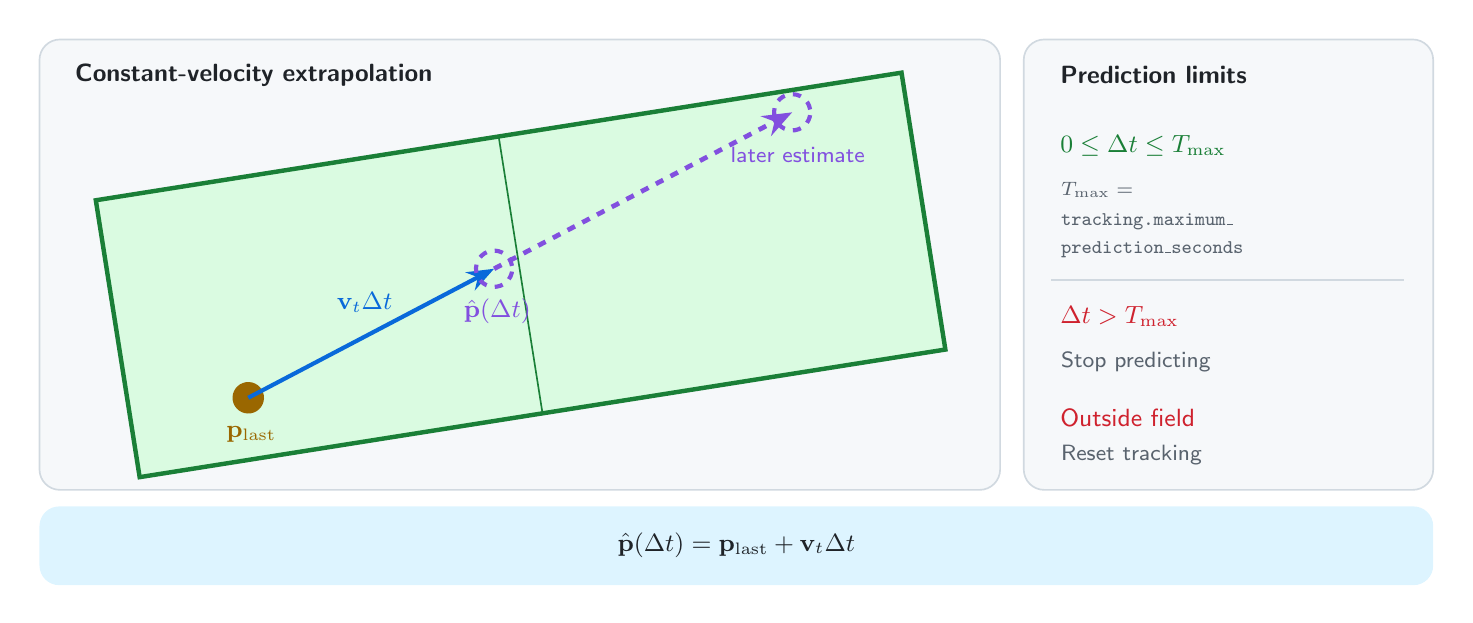
\begin{tikzpicture}[x=1cm, y=1cm]
        \path[use as bounding box] (0, 0) rectangle (18, 7.2);

        % Predicted motion and stopping conditions.
        \draw[card] (0.15, 1.33) rectangle (12.35, 7.05);
        \draw[card] (12.65, 1.33) rectangle (17.85, 7.05);

        \node[heading, anchor=west] at (0.48, 6.6)
            {Constant-velocity extrapolation};
        \node[heading, anchor=west] at (12.99, 6.6)
            {Prediction limits};

        % Extrapolation in the rotated field.
        \begin{scope}[shift={(6.26, 4.06)}, rotate=9]
            \path[fill=ghgreensoft]
                (-5.18, -1.78) rectangle (5.18, 1.78);
            \draw[ghgreen, line width=1.6pt]
                (-5.18, -1.78) rectangle (5.18, 1.78);
            \draw[ghgreen, line width=0.6pt]
                (0, -1.78) -- (0, 1.78);

            \fill[ghorange] (-3.66, -1) circle (0.20);
            \node[mathlabel, anchor=north, text=ghorange]
                at (-3.66, -1.24) {$\mathbf p_{\mathrm{last}}$};

            \draw[bluearrow] (-3.66, -1) -- (-0.32, 0.13);
            \node[mathlabel, text=ghblue, anchor=south]
                at (-2.05, -0.28) {$\mathbf v_t\Delta t$};

            \draw[ghpurple, dashed, -Stealth, line width=1.7pt]
                (-0.32, 0.13) -- (3.73, 1.5);
            \draw[ghpurple, dashed, line width=1.5pt]
                (-0.32, 0.13) circle (0.23);
            \draw[ghpurple, dashed, line width=1.5pt]
                (3.73, 1.5) circle (0.23);

            \node[mathlabel, text=ghpurple, anchor=north]
                at (-0.32, -0.13) {$\hat{\mathbf p}(\Delta t)$};
            \node[note, text=ghpurple, anchor=north]
                at (3.75, 1.17) {later estimate};
        \end{scope}

        % Prediction duration and field constraints.
        \node[regular, anchor=west, text=ghgreen]
            at (12.99, 5.70) {$0\leq\Delta t\leq T_{\max}$};
        \node[tinylabel, anchor=west] at (13, 5.14) {$T_{\max}=$};
        \node[tinylabel, anchor=west] at (13, 4.74)
            {\texttt{tracking.maximum\_}};
        \node[tinylabel, anchor=west] at (13, 4.38)
            {\texttt{prediction\_seconds}};

        \draw[thin] (13, 4) -- (17.48, 4);
        \node[regular, anchor=west, text=ghred]
            at (12.99, 3.53) {$\Delta t>T_{\max}$};
        \node[note, anchor=west] at (13, 2.95) {Stop predicting};
        \node[regular, anchor=west, text=ghred]
            at (12.99, 2.25) {Outside field};
        \node[note, anchor=west] at (13, 1.77) {Reset tracking};

        % Constant-velocity prediction model.
        \path[fill=ghbluesoft, rounded corners=2.5mm]
            (0.15, 0.12) rectangle (17.85, 1.12);
        \node[mathlabel] at (9, 0.63)
            {$\displaystyle\hat{\mathbf p}(\Delta t)=\mathbf p_{\mathrm{last}}+\mathbf v_t\Delta t$};
    \end{tikzpicture}
\end{document}
